\documentclass[a4paper,12pt]{article} 

\usepackage[unicode, pdftex]{hyperref}

% новая команда \RNumb для вывода римских цифр
\newcommand{\RNumb}[1]{\uppercase\expandafter{\romannumeral #1\relax}}

%Добавляет возможность искать и копировать текст
\usepackage{cmap}

%Убирает пробел между названием таблицы/рисунка и самой таблицей/рисунком
\usepackage{caption}
\captionsetup[table]{skip= -0 cm}
\captionsetup[figure]{skip= -0 cm}

%Выравнивание названия таблиц по левому краю
%\usepackage[nooneline]{caption} 
%Размеры отступов 
\usepackage[left=20mm, top=20mm, right=20mm, bottom=20mm, footskip=10mm]{geometry}

%Рисунки
\usepackage{graphicx}
\usepackage{wrapfig} %обтекание элементов
\graphicspath{{graphs}{figures}}  % папки с картинками

%Русский язык в формулах
\usepackage{mathtext}

%  Русский язык
\usepackage[T2A]{fontenc}			
\usepackage[utf8]{inputenc}			
\usepackage[english,russian]{babel}	

%Красная строка для первого абзаца
\usepackage{indentfirst}

%Готические буквы
\usepackage{amssymb}

% Математика
\usepackage{amsmath,amsfonts,amssymb,amsthm,mathtools} 
\usepackage{wasysym}

%Цветные подписи в таблице
\usepackage[table,xcdraw]{xcolor}

%Сделать несколько рядов одним
\usepackage{multirow}

\usepackage{fancyhdr} % Колонтитулы
 	\pagestyle{fancy}
 	\renewcommand{\headrulewidth}{0.3mm}  % Толщина линейки, отчеркивающей верхний колонтитул
 	%\lfoot{Нижний левый}
 	%\rfoot{Нижний правый}
 	\rhead{Белостоцкий Артмемий, Б04-006}
 	%\chead{Верхний в центре}
 	\lhead{Лабораторная работа №5.1.3}
 	\renewcommand{\footrulewidth}{0.3mm}
 	\cfoot{\thepage} % По умолчанию здесь номер страницы
 	
 	
%\captionsetup[table]{
%  position=above,
%  justification=raggedright,
  %labelsep=newline, % <<< label and text on different lines
%  singlelinecheck=false % <<< raggadright also when the cap%tion is shorter
                        % than a single line
%}
 	
\begin{document} 

%Титульник 
\begin{titlepage}
	\begin{center}
		\large 	МИНИСТЕРСТВО ОБРАЗОВАНИЯ И НАУКИ РОССИЙСКОЙ ФЕДЕРАЦИИ\\
				МОСКОВСКИЙ ФИЗИКО-ТЕХНИЧЕСКИЙ ИНСТИТУТ \\
				(НАЦИОНАЛЬНЫЙ ИССЛЕДОВАТЕЛЬСКИЙ ИНСТИТУТ)\\ 
				ФИЗТЕХ-ШКОЛА ЭЛЕКТРОНИКИ, ФОТОНИКИ \\
				И МОЛЕКУЛЯРНОЙ ФИЗИКИ \\
		
		
		\vspace{4.0 cm}
		Лабораторная работа № 5.1.3 \\ 
		\LARGE \textbf{Эффект Рамзауэра}
	\end{center}
	\vspace{3 cm} \large
	
	\begin{flushright}
		выполнил студент 3 курса \\
		{группы Б04-006}\\
		\textbf{Белостоцкий Артемий}\\
	\end{flushright}
	
	\vfill

	\begin{center}
	Долгопрудный, 2022 г.
	\end{center}
\end{titlepage}                                                                      

\section*{Аннотация}

В данной работе исследуется энергетическая зависимость вероятности рассеяния электронов атомами ксенона, определяются энергии электронов, при которых наблюдается <<просветление>> ксенона, и оценивается размер его внешней электронной оболочки.

\section*{Теоретические сведения}

Рассмотрим рассеяние электрона на одномерной потенциальной яме глубины $U_0$.

\begin{figure}[h]
	\centering
	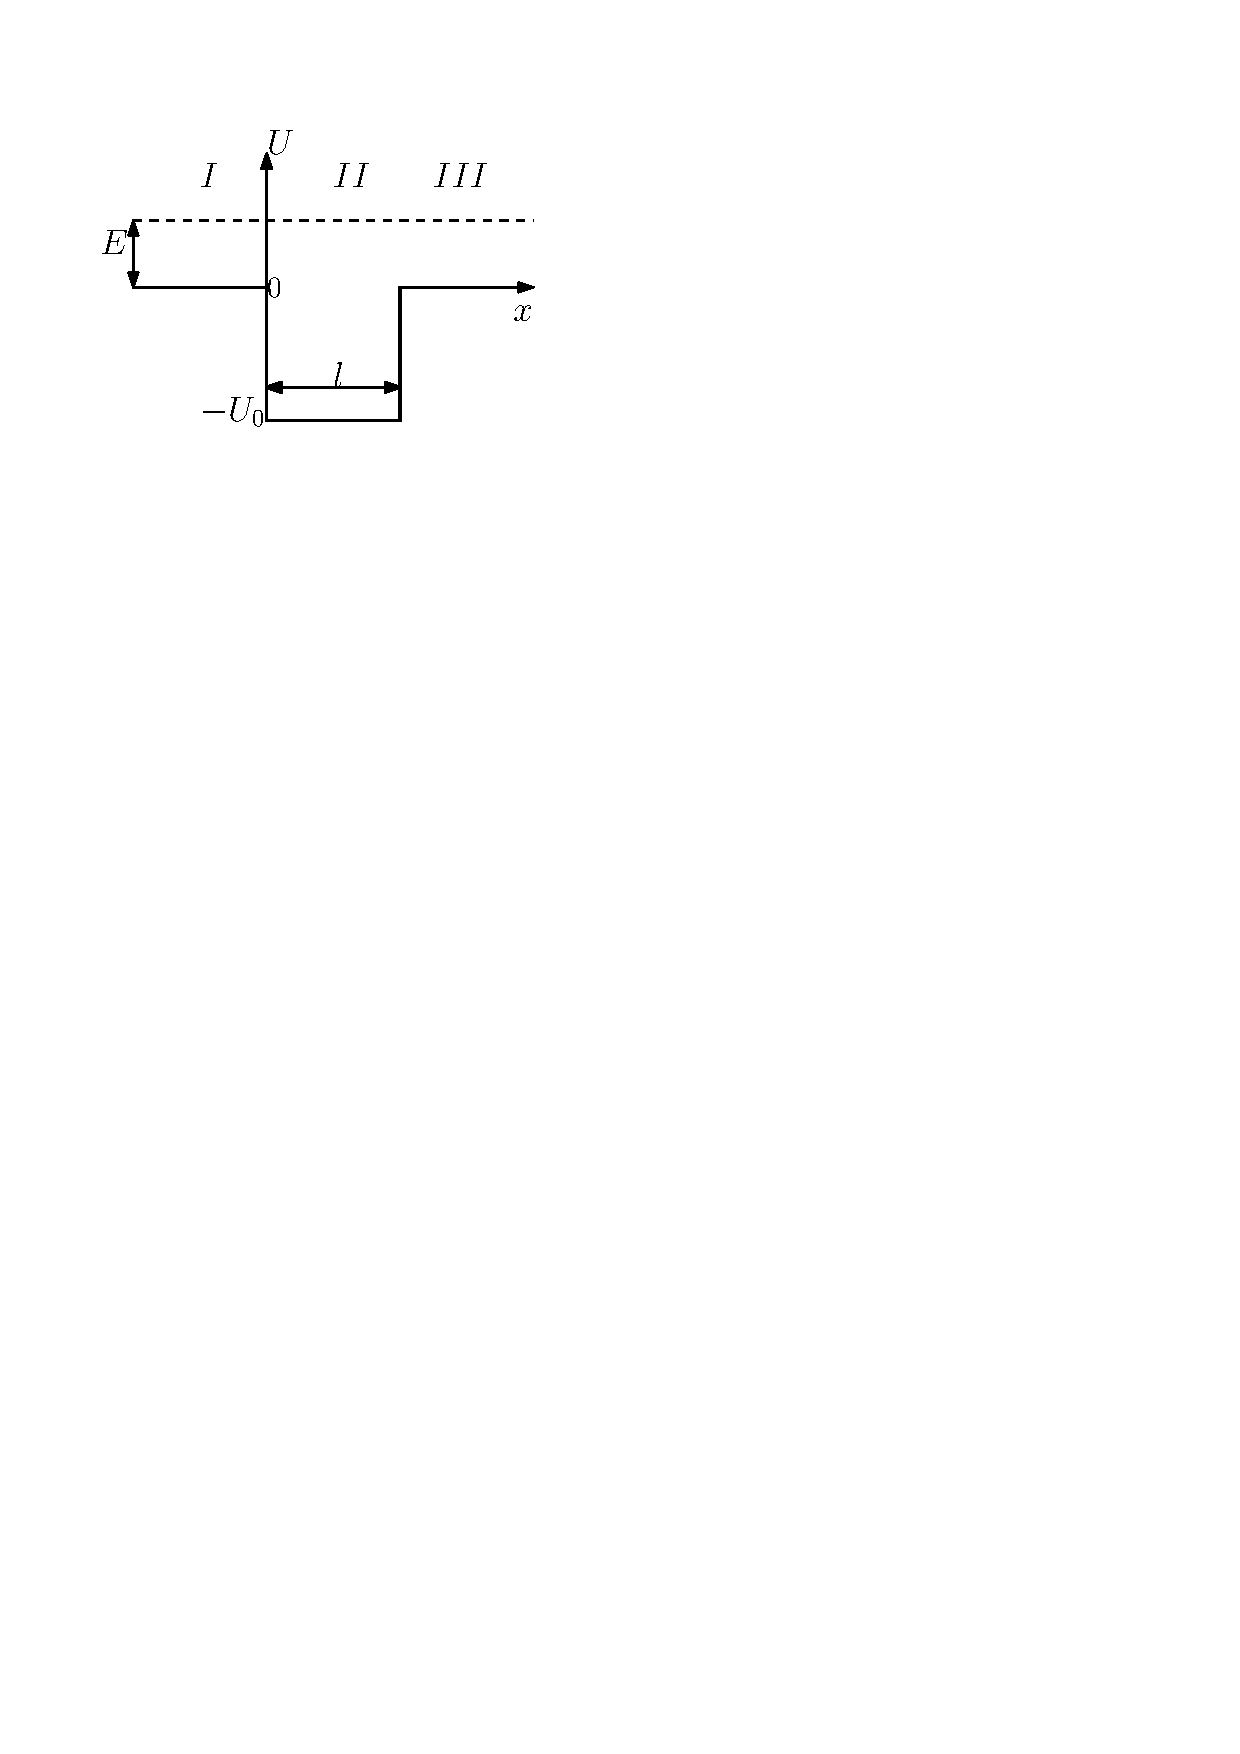
\includegraphics[width=0.5\linewidth]{fig1}
	\caption{Схематичное изображение прямоугольной ямы, над которой пролетает частица с энергией $E$}
	\label{fig1:potential_well}
\end{figure}

Разделим все пространство на 3 области -- <<до ямы>> , <<в яме>>, <<после ямы>>. Для каждой из областей запишем стационарное уравнение Шредингера, чтобы найти $\psi$-функцию, описывающую состояние электрона в каждой области.

\begin{align*}
	\begin{cases}
	\psi^{\prime \prime}_{\RNumb{1}} + k_1^2 \psi_{\RNumb{1}} &= 0, \quad k_1^2 = \frac{2m}{\hbar^2}E \\
	%
	\psi^{\prime \prime}_{\RNumb{2}} + k_2^2 \psi_{\RNumb{2}} &= 0, \quad k_2^2 = \frac{2m}{\hbar^2}(E+U_0) \\
	%
	\psi^{\prime \prime}_{\RNumb{3}} + k_3^2 \psi_{\RNumb{3}} &= 0, \quad k_3^2 = \frac{2m}{\hbar^2}E
	\end{cases}
\end{align*}

Тогда решения этих уравнений:

\begin{align*}
	\begin{cases}
		\psi_{\RNumb{1}} = e^{ik_1x} + r e^{-ik_1x} \\
		%
		\psi_{\RNumb{2}} = A e^{ik_2x} + B e^{-ik_2x} \\
		%
		\psi_{\RNumb{3}} = d e^{ik_3x} + c e^{-ik_3x}
	\end{cases}
\end{align*}

Заметим, что в области $\RNumb{3}$ нет физических предпосылок к отражению, следовательно $c=0$. Оставшиеся константы определим из условия гладкости и непрерывности $\psi$-функции на границах областей.

\begin{align} \label{eq1:initial_cond}
	\begin{cases}
		\psi_{\RNumb{1}} (0) = \psi_{\RNumb{2}} (0) \\
		%
		\psi^{\prime}_{\RNumb{1}} (0) = \psi^{\prime}_{\RNumb{2}} (0) \\
		%
		\psi_{\RNumb{2}} (l) = \psi_{\RNumb{3}} (l) \\
		%
		\psi^{\prime}_{\RNumb{2}} (l) = \psi^{\prime}_{\RNumb{3}} (l) \\
	\end{cases}
\end{align}

\newpage

Введем определение коэффициента прохождения электронов.

\begin{align*}
	D = \frac{j_{прош}}{j_{пад}},
\end{align*}

где $j$ -- плотность потока вероятности, соответственно, падающих и прошедших частиц.

\begin{align} \label{eq2:current}
	j \stackrel{def}{=} \frac{i \hbar}{2m} (\psi \nabla \psi^* - \psi^* \nabla \psi) = \frac{i \hbar}{2m} (\psi {\psi^*}^{\prime} - \psi^* \psi^{\prime})
\end{align}

Тогда, с учетом (\ref{eq1:initial_cond}), (\ref{eq2:current}) и того, что $k_1 = k_2$, получим:

\begin{align} \label{eq3:coef_of_transmission}
	D = \frac{16 k_1^2 k_2^2}{16 k_1^2 k_2^2 + 4(k_1^2 - k_2^2)^2 \sin ^2 (k_2 l)} 
\end{align}

Тогда условия максимума и минимума $D$ имеют вид:

\begin{align} \label{eq4:max_energy} 
	k_2 l \approx \sqrt{E_{max} + U_0} \frac{l}{1,95} = \pi n \
\end{align}

\begin{align*}
	k_2 l \approx \sqrt{E_{min} + U_0} \frac{l}{1,95} = \frac{\pi}{2} + \pi n 
\end{align*}

Поделим уравнения друг на друга и вычтем одно из другого получим:

\begin{align} 
	\frac{E_{min} + U_0}{E_{max} + U_0} = \left(1 + \frac{1}{2n} \right)^2  \label{eq5:to_find_U} \\
	\sqrt{E_{min} - E_{max}} \frac{l}{1,95} = \sqrt{ \frac{\pi^2}{4} + \pi^2 n} \label{eq6:to_find_l}
\end{align}

Заметим, что данные формулы справедливы для размерных величин: $l[\mathring{A}]$, $(E + U_0)$[эВ]

\newpage

\section*{Экспериментальная установка}
\begin{figure}[h]
	\centering
	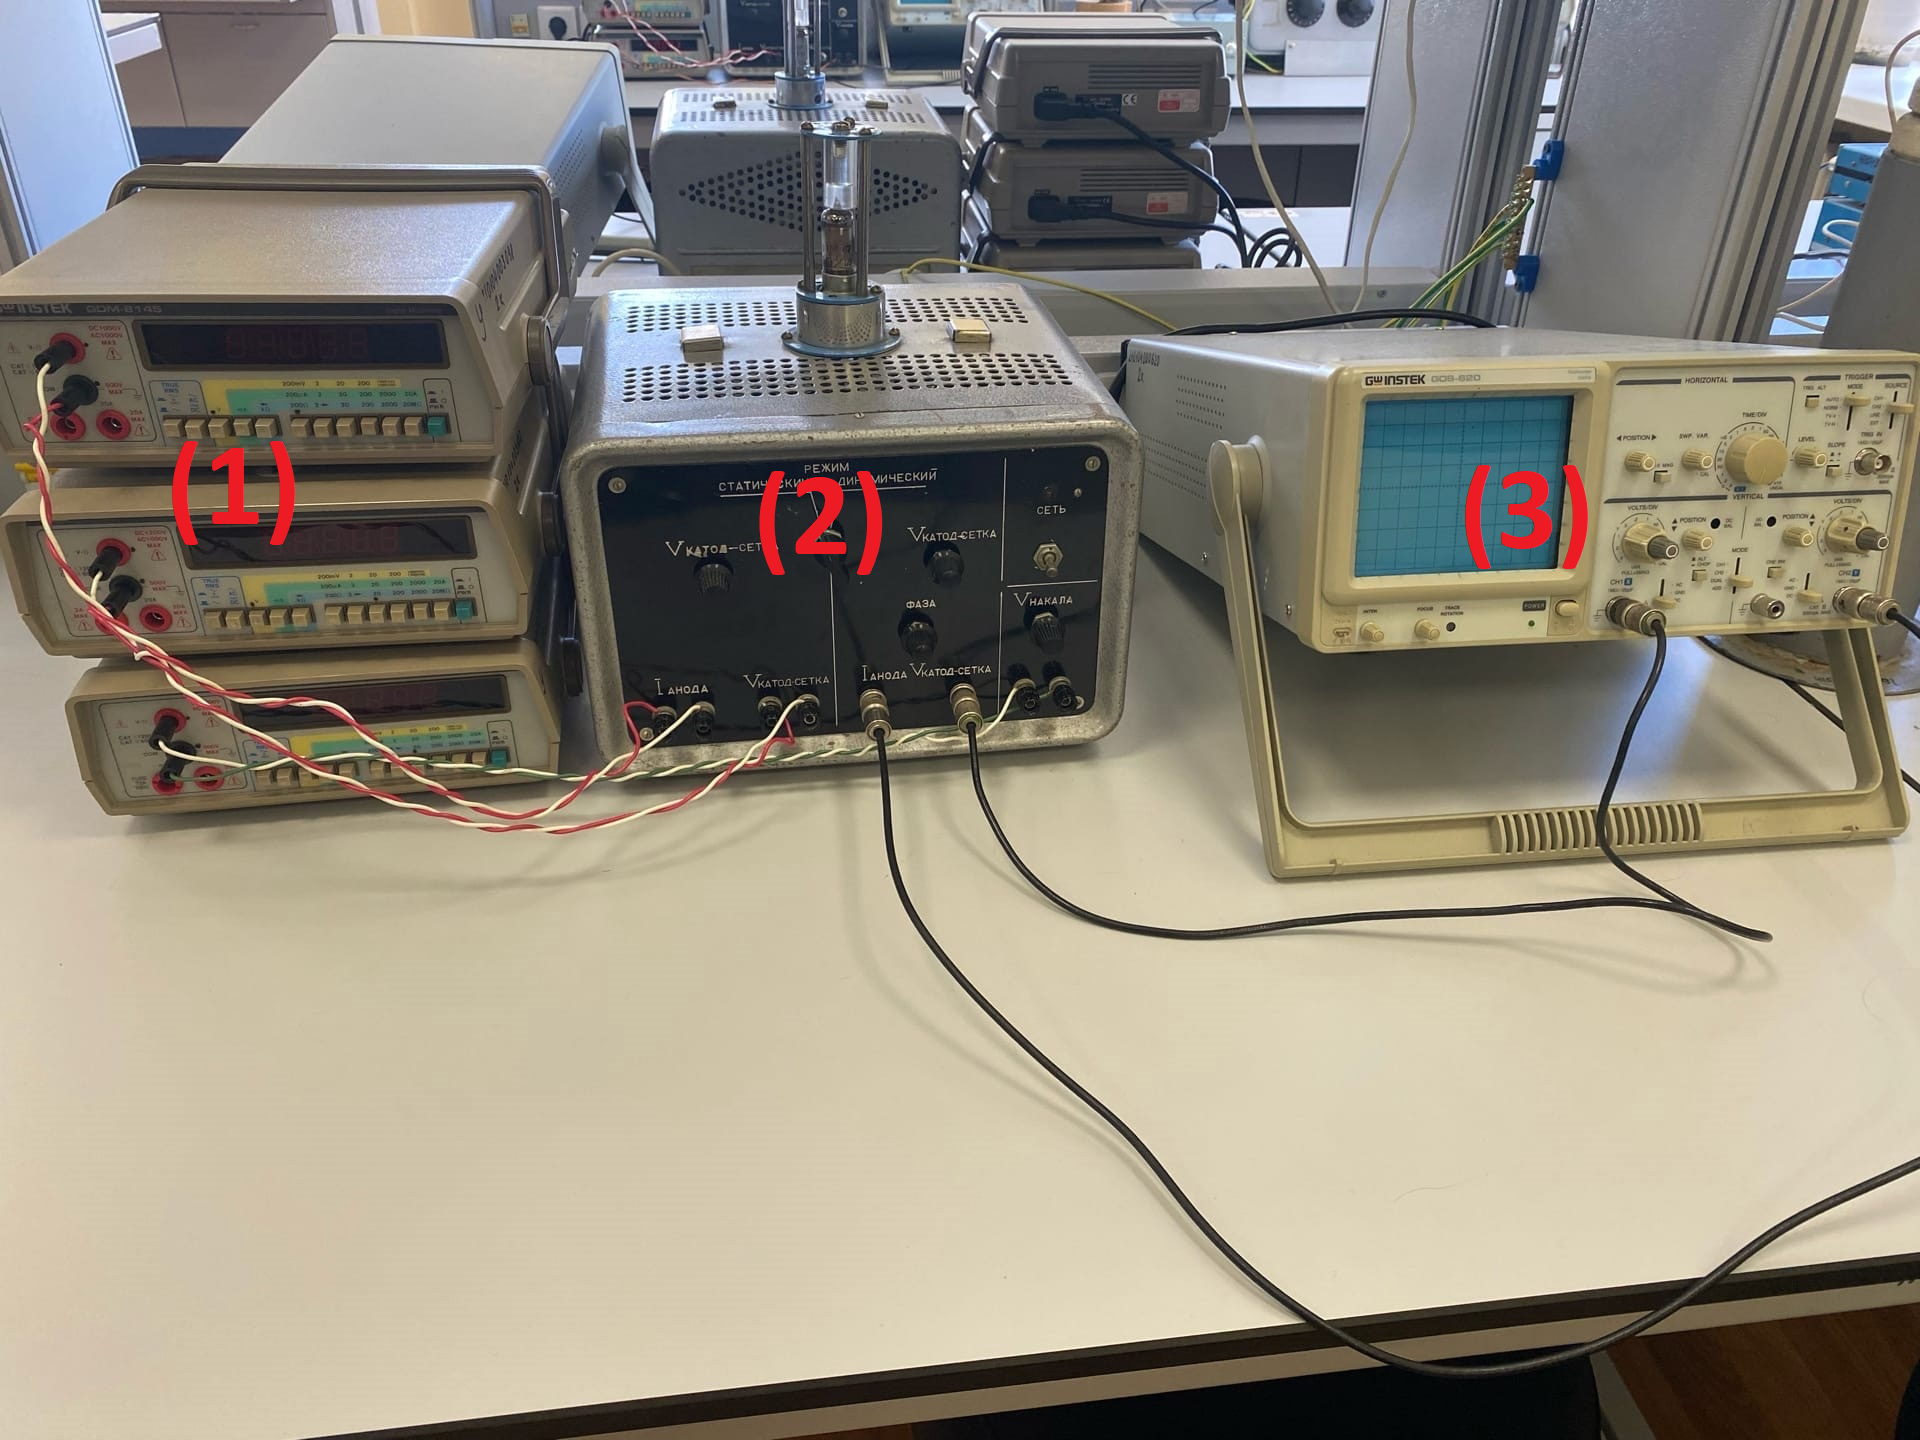
\includegraphics[width=0.7\linewidth]{fig4}
	\caption{Экспериментальная установка. (1) -- вольтметры, (2) -- Блок источников питания, (3) -- осциллограф}
\end{figure}

\begin{figure}[h!]
	\centering
	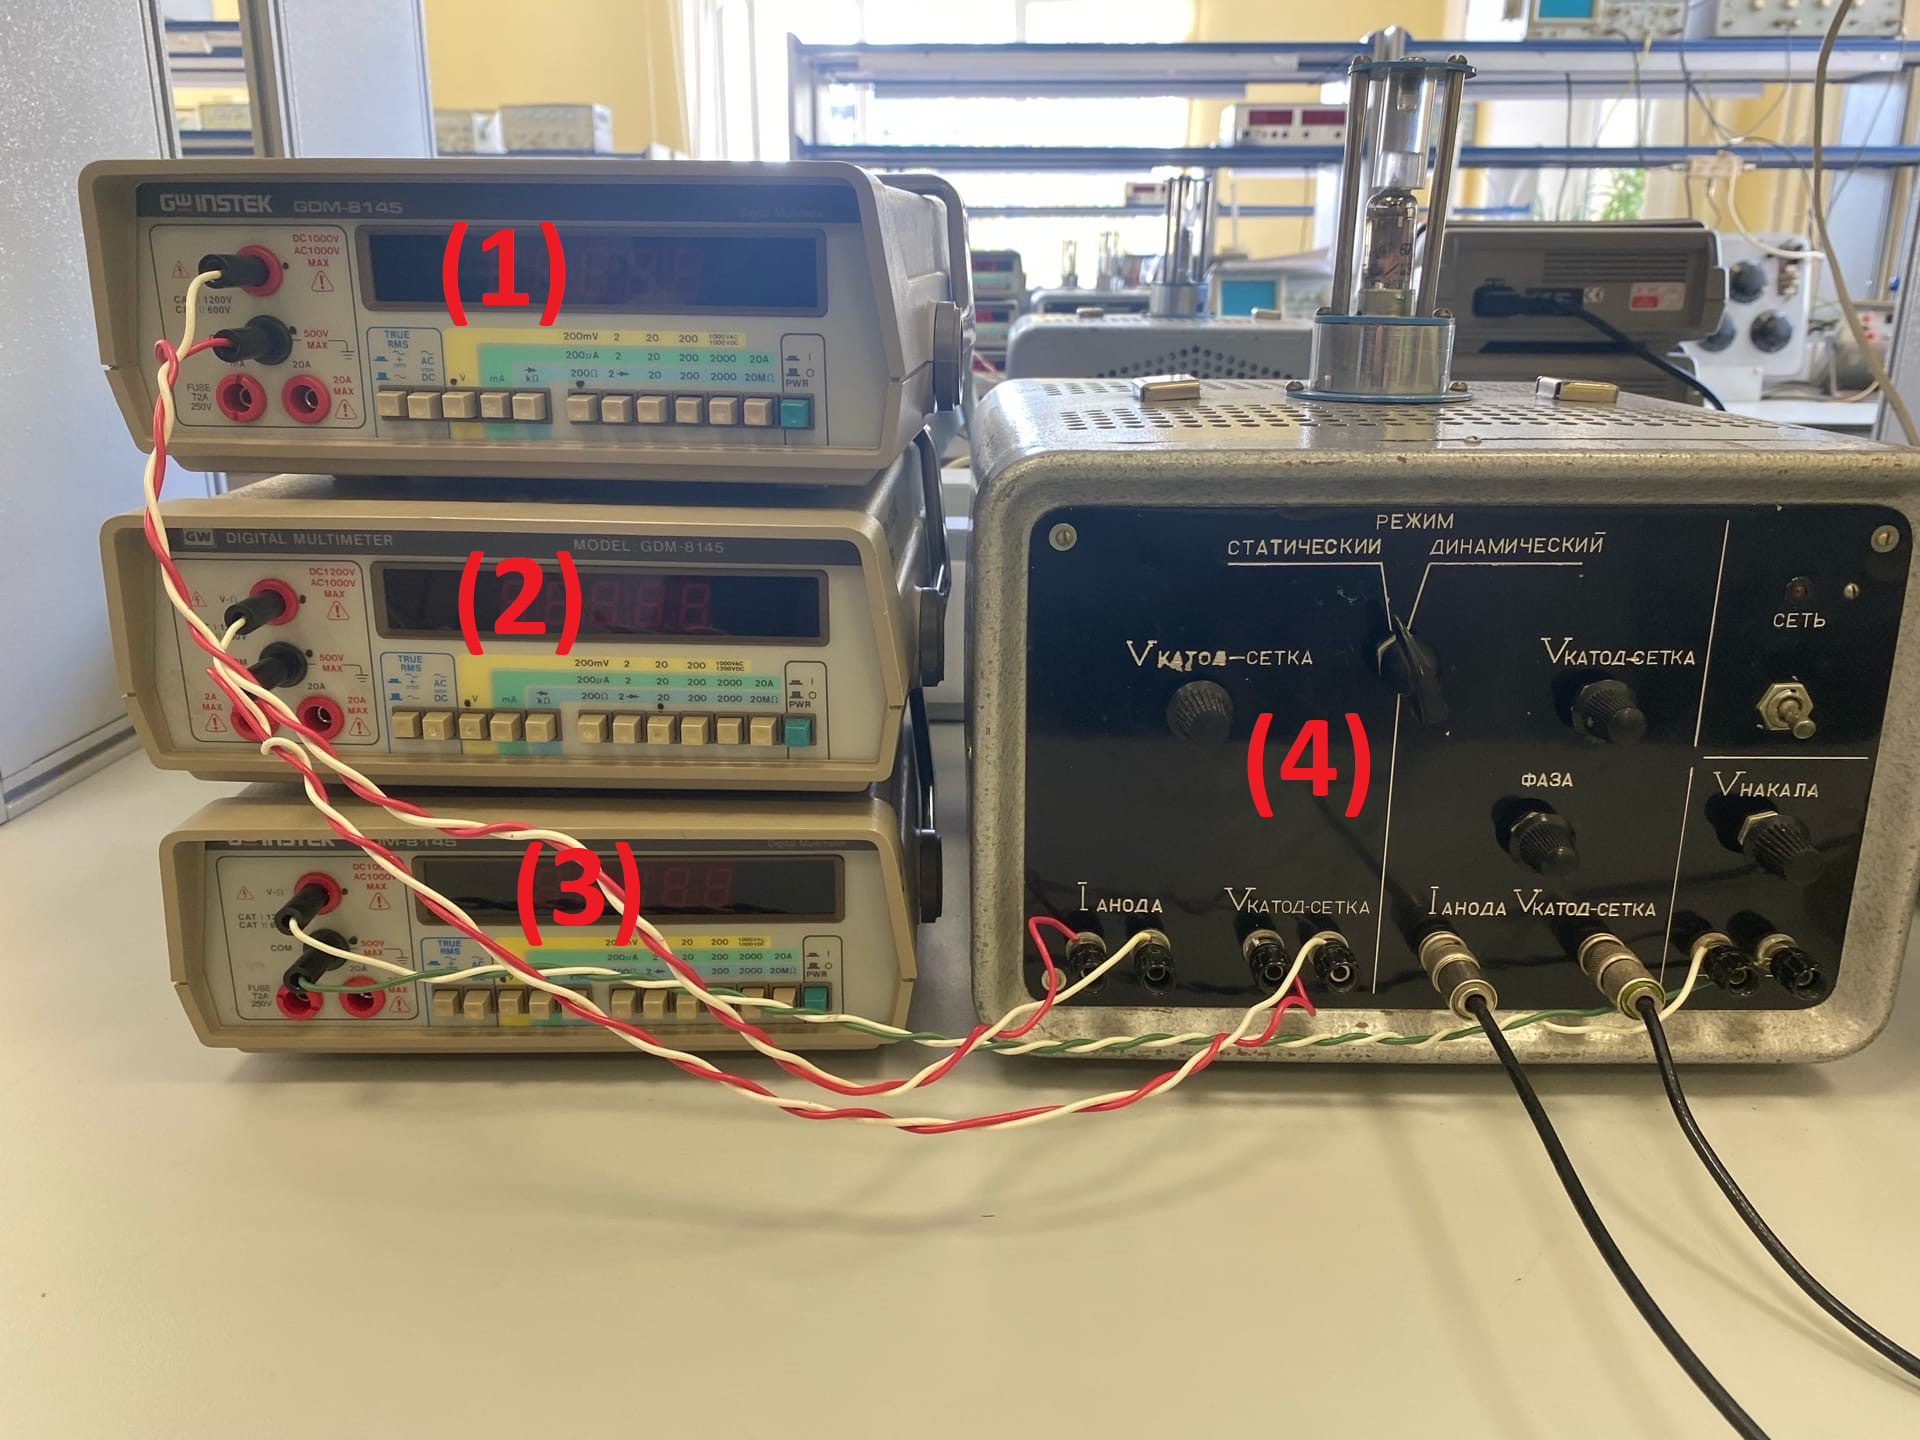
\includegraphics[width=0.7\linewidth]{fig5}
	\caption{Экспериментальная установка.(1) -- Вольтметр, снимающий показания с анода, (2) -- Вольтметр, снимающий показания с катода, Вольтметр, снимающий показания напряжения накала, (4) -- БИП с ручками управления напряжения катода, напряжения накала и тумблером переключения режимов.}
\end{figure}

\section*{Ход работы}

Используя формулы (\ref{eq6:to_find_l}), (\ref{eq5:to_find_U}) мы сможем оценить ширину и глубину нашей <<ямы>>. В нашем случае, удается наблюдать лишь один минимум и максимум ($n=1$).

\subsubsection*{Динамический режим}

При максимальном ускоряющем напряжении получим ВАХ тиратрона на экране осциллографа при двух различных напряжениях накала.

Осциллограммы представлены на Рис. \ref{fig2:Osc_1}, \ref{fig3:Osc_2}.

\begin{figure}[h]
	\centering
	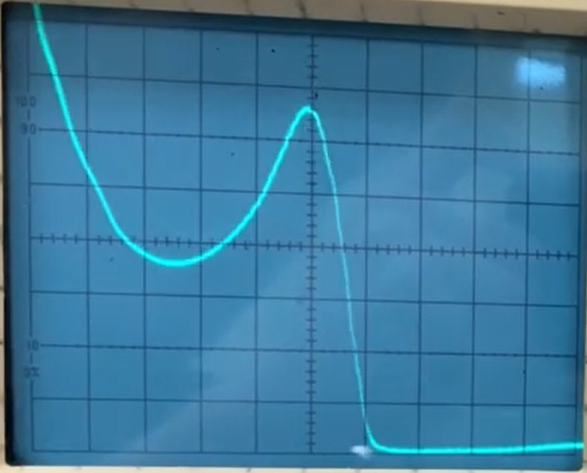
\includegraphics[scale=0.9]{fig2}
	\caption{ВАХ тиратрона при напряжении накала -- $U_н = 2,99 В$}
	\label{fig2:Osc_1}
\end{figure}

\begin{figure}[h!]
	\centering
	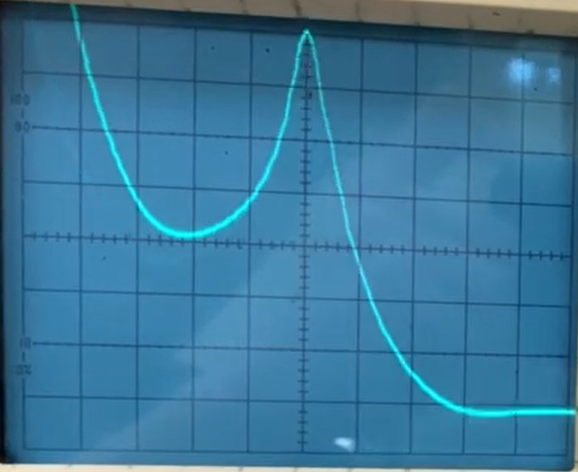
\includegraphics[scale=0.9]{fig3}
	\caption{ВАХ тиратрона при напряжении накала -- $U_н = 2,99 В$}
	\label{fig3:Osc_2}
\end{figure}

По ВАХ определим максимальное ($V_{max}$) и минимальное ($V_{min}$) напряжение, а также напряжение пробоя ($V_{пробой}$). Полученные данные занесем в Таблицы \ref{table1:voltage1} и \ref{table2:voltage2}

\begin{table}[h]
\centering
\caption{Измерения по осциллограмме при $U_н = 2,99В$}
\label{table1:voltage1}
\begin{tabular}{|c|c|c|c|}
\hline
\textbf{$V_{max}$, В} & \textbf{$V_{min}$, В} & \textbf{$V_{пробой}$,В} & \textbf{$\sigma_V$, В} \\ \hline
1,6 & 6,0 & \multirow{2}{*}{23,1} & 0,4 \\ \cline{1-2} \cline{4-4} 
1,6 & 6,6 &  & 0,4 \\ \hline
\end{tabular}
\end{table}

\begin{table}[h]
\centering
\caption{Измерения по осциллограмме при $U_н = 2,5В$}
\label{table2:voltage2}
\begin{tabular}{|c|c|c|c|}
\hline
\textbf{$V_{max}$, В} & \textbf{$V_{min}$, В} & \textbf{$V_{пробой}$,В} & \textbf{$\sigma_V$, В} \\ \hline
1,6 & 7,1 & \multirow{2}{*}{22,6} & 0,4 \\ \cline{1-2} \cline{4-4} 
1,6 & 6,4 &  & 0,4 \\ \hline
\end{tabular}
\end{table}

По формуле (\ref{eq5:to_find_U}) найдем $U_0$

\begin{align*}
	U_0 = (2,34 \pm 1,51) эВ,
\end{align*}

где значение $U_0$ -- средняя величина, а ее погрешность рассчитывалась по формуле:

\begin{align*}
	\sigma_{случ} = \sqrt{ \frac{1}{4 \times 3} \sum \limits_{i=1}^{4} (U_{0i} - \overline{U_0})^2 } \approx 0,1 эВ \\
	\sigma_{сист} = \sqrt{4 * \sigma^2_{U_{0i}}} = 2 \sigma_{U_{0i}} = 2 \frac{\sqrt{97}}{5} \sigma_{V} \approx 1,51 эВ \\
	\sigma_{полн} = \sqrt{\sigma^2_{случ} + \sigma^2_{сист}} \approx 1,51 эВ
\end{align*}

По формуле (\ref{eq6:to_find_l}) найдем $l$:

\begin{align*}
	l = (3,09 \pm 0,04) \mathring{A}
\end{align*}

где значение $l$ -- средняя величина, а ее погрешность рассчитывалась по формуле:

\begin{align*}
	\sigma_{случ} = \sqrt{ \frac{1}{4 \times 3} \sum \limits_{i=1}^{4} (l_{i} - \overline{l})^2 } \approx 0,015 \mathring{A} \\
	\sigma_{сист} = \sqrt{\sum \limits_{i=1}^{4} \frac{\sigma^2_V}{4 (E_{min_i} - E_{max_i})^{3/2}}} \approx 0,037 \mathring{A}\\
	\sigma_{полн} = \sqrt{\sigma^2_{случ} + \sigma^2_{сист}} \approx 0,04 \mathring{A} 
\end{align*}

Потенциал ионизации равен напряжению пробоя:

$$
	U \approx 22,9 эВ
$$

\newpage

\subsubsection*{Статический режим}

Переведем переключатель в положение <<Статич.>> и проведем измерение ВАХ тиратрона для двух значений напряжения накала. Полученные данные представлены в Таблицах \ref{table3:VAC_1}, \ref{table3:VAC_2}

По полученным данным построим зависимость анодного тока от напряжения на катоде $I_a = f(V_c)$, учитывая что $\sigma_{I_a} = 10^{-7} мА$, $\sigma_{V_c} = 0,1 В$

\begin{figure}[h]
	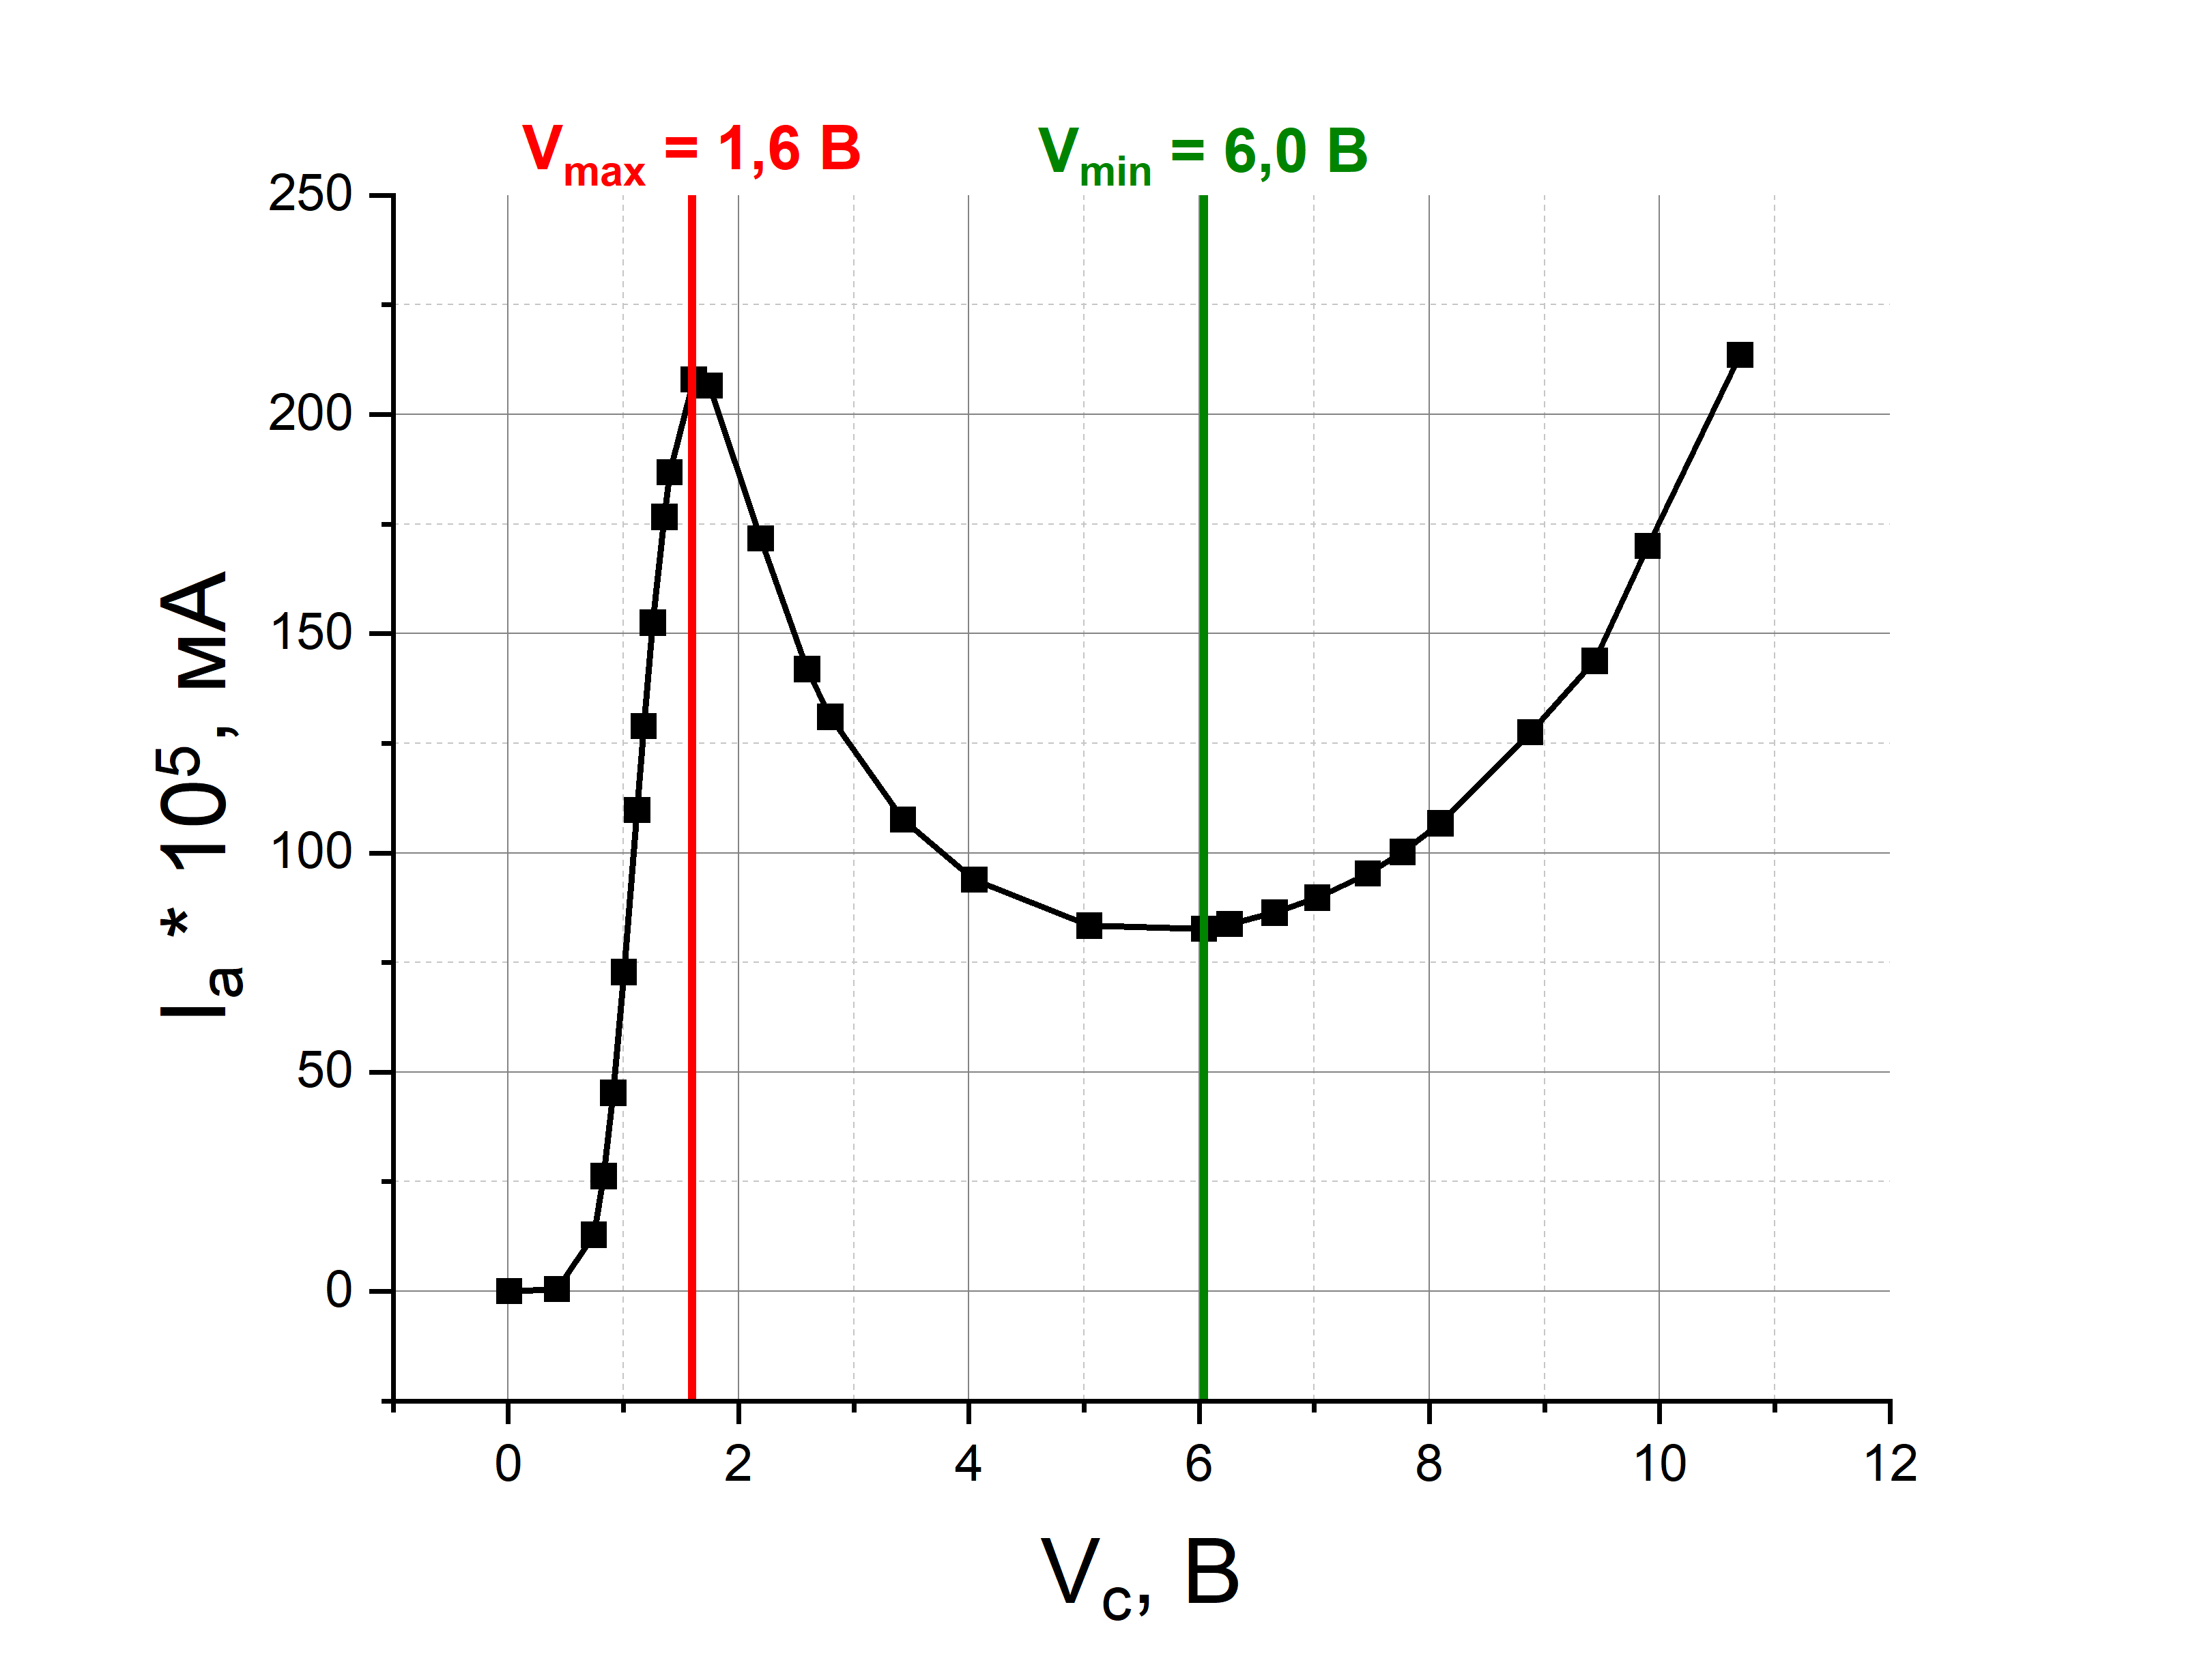
\includegraphics[width=\linewidth]{graph1}
	\caption{Зависимость анодного тока от напряжения на катода при напряжении накала $U=2,51В$}
	\label{graph1:VAC_1}
\end{figure}

\newpage

\begin{figure}[h]
	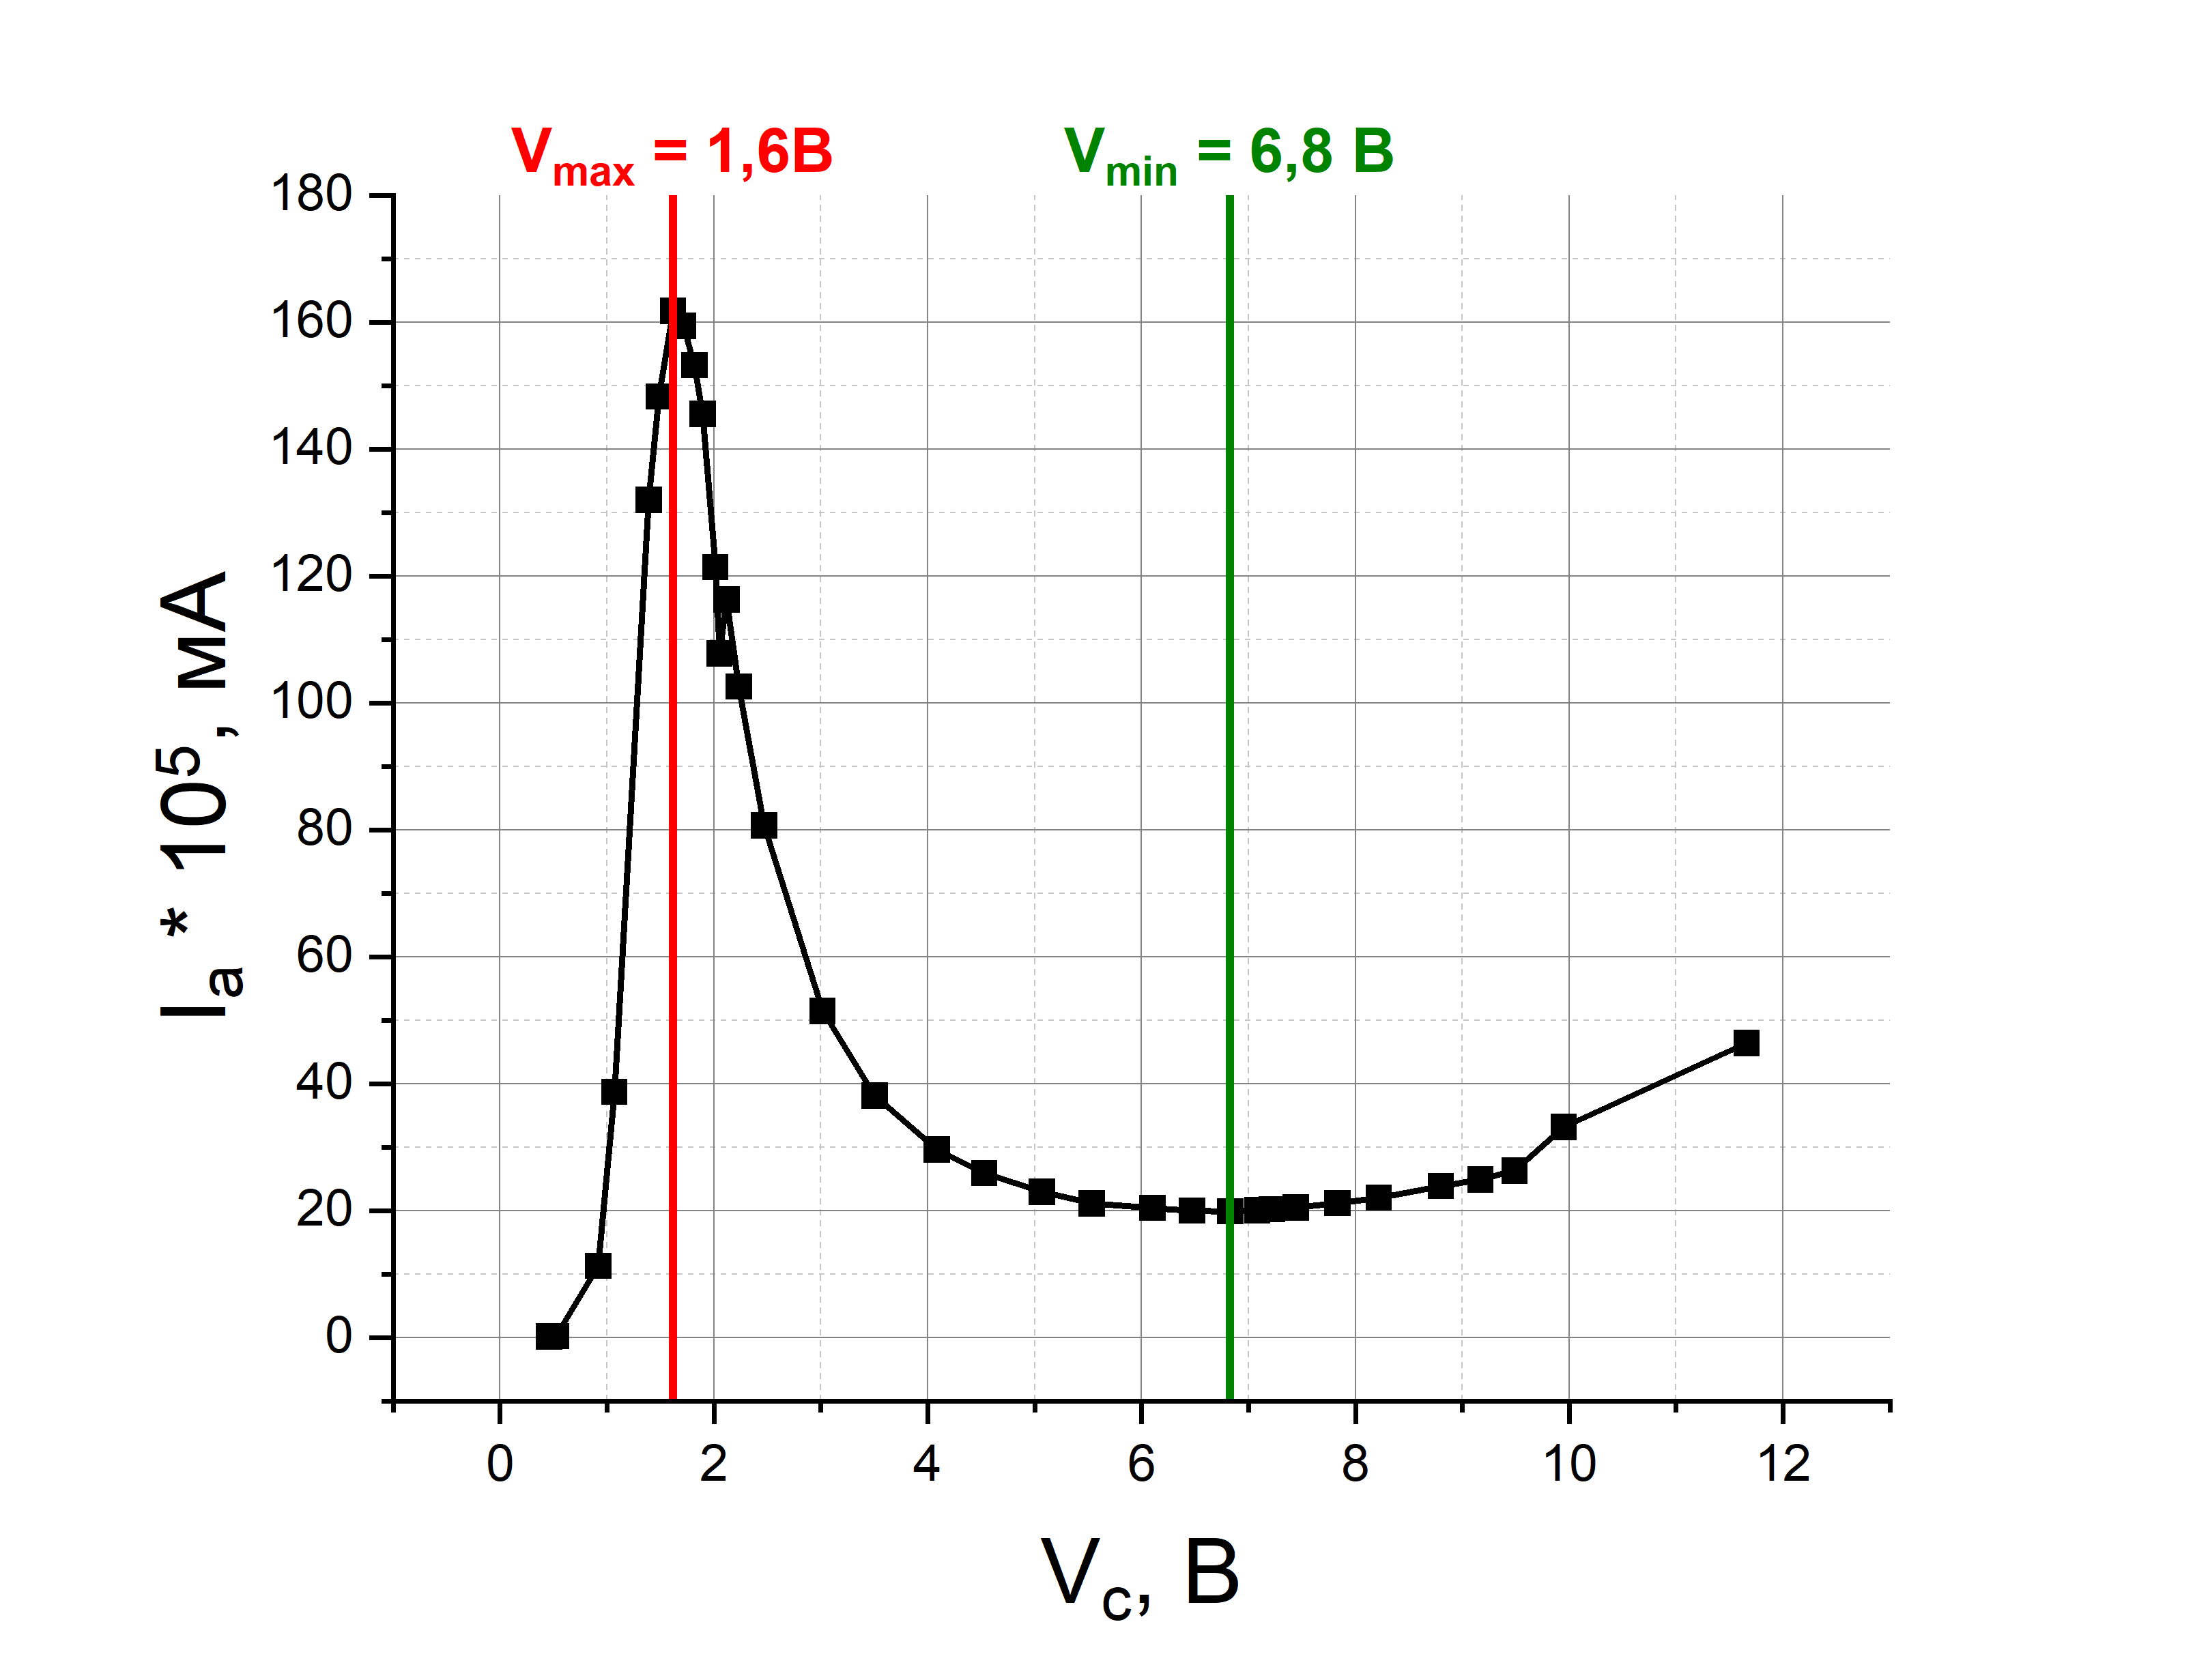
\includegraphics[width=\linewidth]{graph2}
	\caption{Зависимость анодного тока от напряжения на катода при напряжении накала $U=3,02В$}
	\label{graph2:VAC_2}
\end{figure}

Проведем аналогичные расчеты для $U_0$ и $l$, взяв данные из графиков. Получим:

\begin{align*}
	U_0 = (2,24 \pm 0,41) эВ \\
	l = (3,13 \pm 0,03) \mathring{A}
\end{align*}

Из формулы (\ref{eq4:max_energy}) оценим напряжения, при которых должны появляться максимумы второго и третьего порядков:

\begin{align*}
	E_2 = \left(\frac{2\pi \times 1,95}{3}\right)^2 - 2,2 \approx 14 эВ \\ 
	E_3 = \left(\frac{3\pi \times 1,95}{3}\right)^2 - 2,2 \approx 36 эВ \\
\end{align*}

Данных максимумов в работе не наблюдается, так как рабочий диапазон измерений лежит до 11 В, а при напряжениях более 22 В газ ионизуется и происходит пробой, вследствие чего измерить максимумы так же не представляется возможным.

В завершении, построим график зависимости вероятности рассеяния электронов от энергии на основе формулы:

$$
	w(V) = -\frac{1}{C} \ln \frac{I_a(V)}{I_0}
$$

\newpage

\begin{figure}[h]
	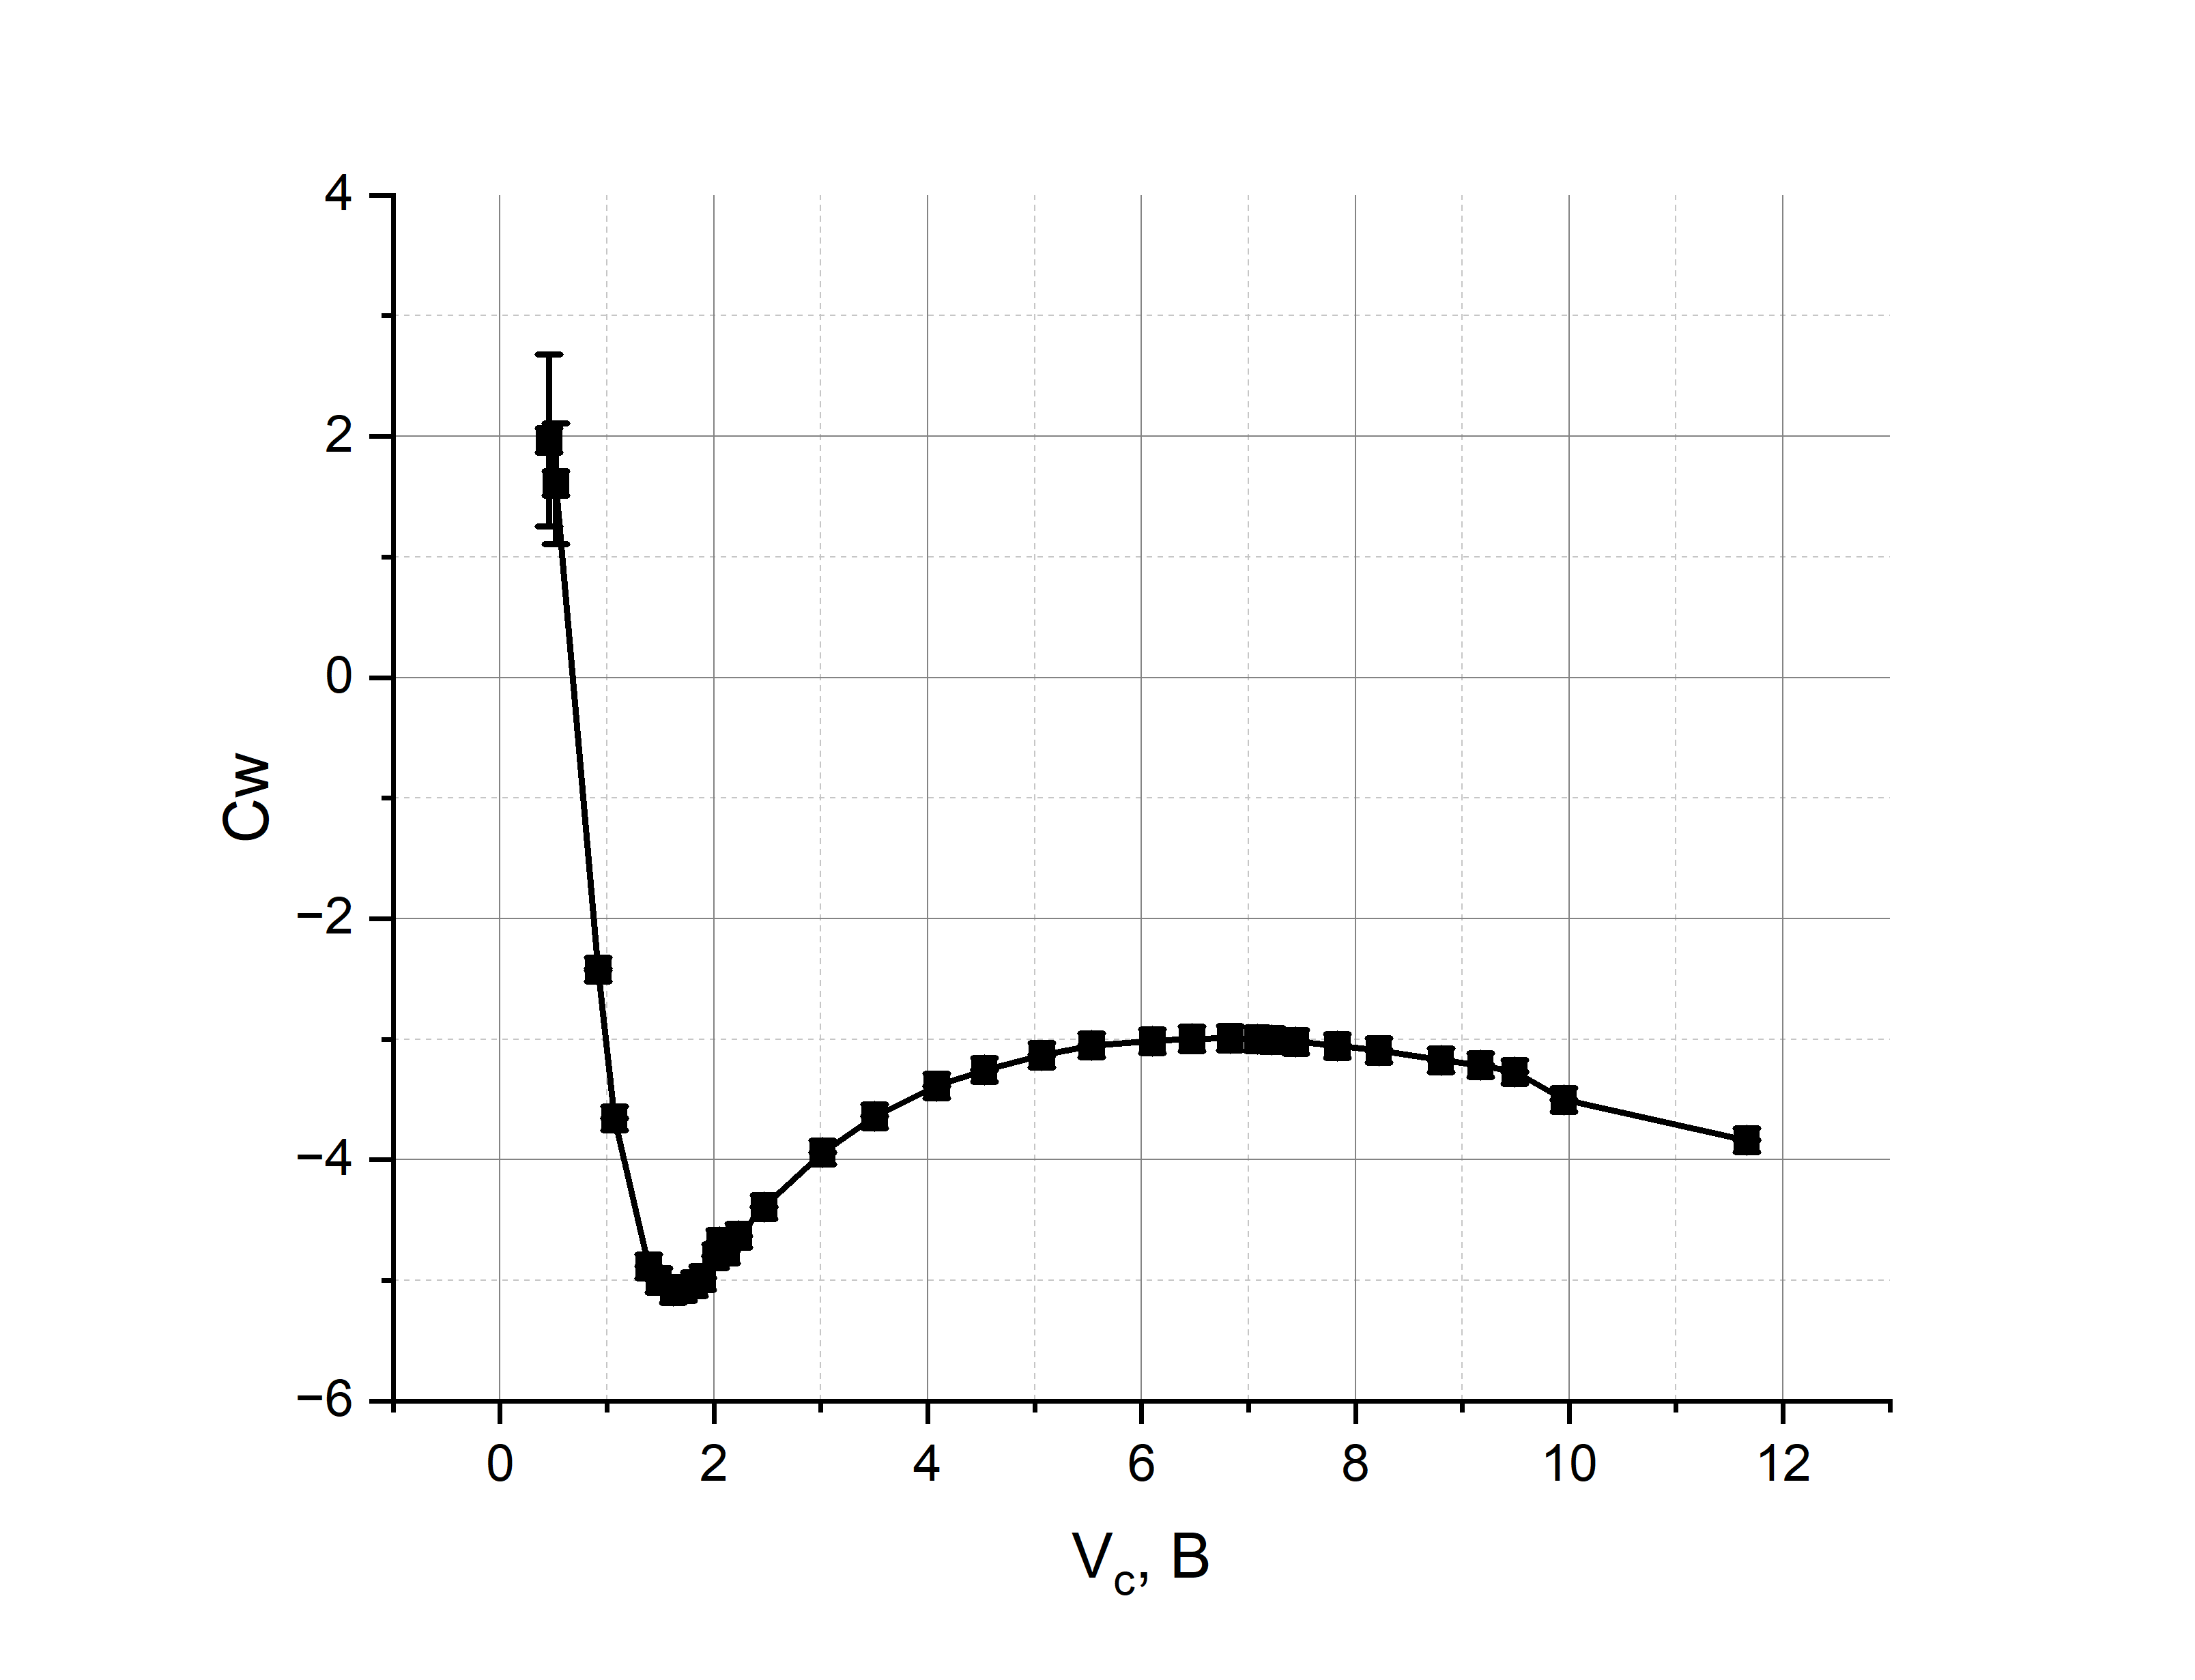
\includegraphics[width=\linewidth]{graph3}
	\caption{Зависимость вероятности рассеяния электрона от его энергии (с точностью до константы)}
	\label{graph3:Probability}
\end{figure}

\section*{Обсуждение результатов}

Заметим, что реальная яма в физическом эффекте Рамзауэра трехмерная. Проверим, в модели трехмерной сферически симметричной ямы (Рис (\ref{fig4:potential_well_shere})), будут ли в ней связанные состояния при полученных параметрах ямы ($U_0 \approx 2 эВ, l = 3 \mathring{A}$).

Условие существования связанных состояний в такой яме:

\begin{align*}
	U_0 \left( \frac{l}{2} \right)^2 &\geqslant \frac{\pi^2 \hbar^2}{8 m} \\
	8 &\geqslant 15 - неверно
\end{align*}

Следовательно, связанные состояния не существуют.   

\begin{figure}[h!]
	\centering
	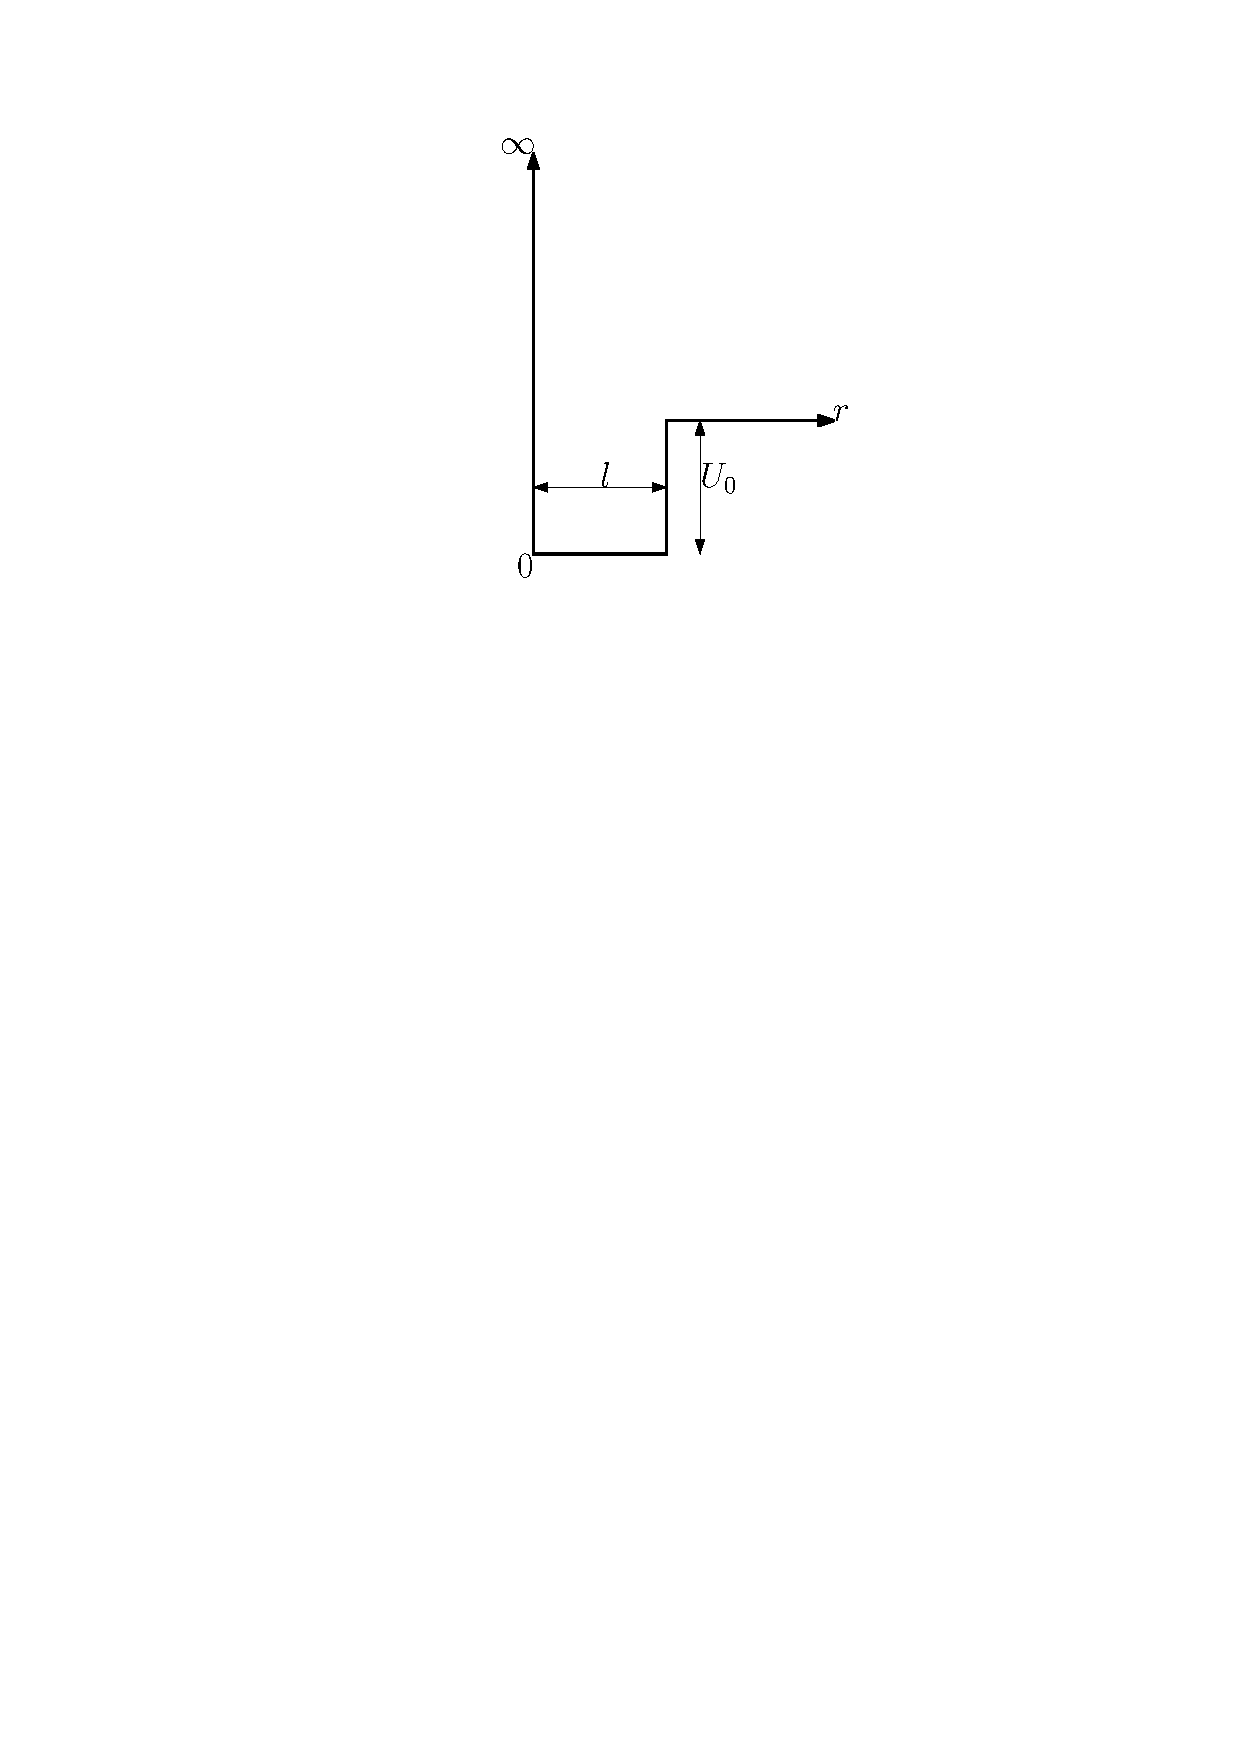
\includegraphics[width=0.5\linewidth]{fig6}
	\caption{Схематичное изображение сферически симметричной прямоугольной ямы}
	\label{fig4:potential_well_shere}
\end{figure}

\pagebreak

\section*{Выводы}

\begin{itemize}
\item В ходе работы был получен ионизационный потенциал газа, находящегося в тиратроне -- $U \approx 23 эВ$. Заметим, что потенциал ионизации воздуха $\approx 39 эВ$, следовательно, можно предположить, что в тиратроне находится смесь воздуха с каким-то газом.

\item Также были получены характеристики атомов газа: глубина потенциальной ямы и ее ширина двумя разными способами. Заметим, что погрешность статического метода оказалась меньше.

\begin{table}[h]
\centering
\begin{tabular}{|c|c|c|}
\hline
 & Статический & Динамический \\ \hline
$U_0$, эВ & $2,24 \pm 0,41$ & $2,34 \pm 1,51$ \\ \hline
l, $\mathring{A}$ & $3,13 \pm 0,03$ & $3,09 \pm 0,04$ \\ \hline
\end{tabular}
\end{table}
\end{itemize}
\newpage

\section*{Приложение}

\begin{table}[h]
\centering
\caption{Зависимость анодного тока от напряжения на катоде при напряжении накала U=2,51В}
\label{table3:VAC_1}
\begin{tabular}{|c|c|}
\hline
$I_a *10^5$, мА & $V_c$, В \\ \hline
0,14 & 0,46 \\ \hline
0,20 & 0,52 \\ \hline
11,28 & 0,92 \\ \hline
38,72 & 1,07 \\ \hline
132,00 & 1,39 \\ \hline
148,28 & 1,48 \\ \hline
161,75 & 1,62 \\ \hline
159,43 & 1,71 \\ \hline
153,20 & 1,82 \\ \hline
145,54 & 1,90 \\ \hline
121,40 & 2,01 \\ \hline
107,80 & 2,05 \\ \hline
116,30 & 2,12 \\ \hline
102,60 & 2,23 \\ \hline
80,70 & 2,47 \\ \hline
51,43 & 3,01 \\ \hline
38,10 & 3,51 \\ \hline
29,60 & 4,09 \\ \hline
25,90 & 4,53 \\ \hline
22,94 & 5,07 \\ \hline
21,15 & 5,54 \\ \hline
20,41 & 6,10 \\ \hline
20,01 & 6,47 \\ \hline
19,90 & 6,83 \\ \hline
20,06 & 7,08 \\ \hline
20,21 & 7,22 \\ \hline
20,51 & 7,44 \\ \hline
21,20 & 7,83 \\ \hline
22,04 & 8,22 \\ \hline
23,89 & 8,80 \\ \hline
24,91 & 9,17 \\ \hline
26,30 & 9,49 \\ \hline
33,17 & 9,95 \\ \hline
46,40 & 11,66 \\ \hline
\end{tabular}
\end{table}

\newpage

\begin{table}[h]
\centering
\caption{Зависимость анодного тока от напряжения на катоде при напряжении накала U=3,01В}
\label{table3:VAC_2}
\begin{tabular}{|c|c|}
\hline
$I_a *10^5$, мА & $V_c$, В \\ \hline
0,52 & 0,42 \\ \hline
12,90 & 0,74 \\ \hline
26,30 & 0,83 \\ \hline
45,30 & 0,91 \\ \hline
72,81 & 1,00 \\ \hline
109,80 & 1,12 \\ \hline
128,90 & 1,18 \\ \hline
152,50 & 1,26 \\ \hline
176,60 & 1,36 \\ \hline
186,80 & 1,40 \\ \hline
208,00 & 1,61 \\ \hline
206,60 & 1,75 \\ \hline
171,70 & 2,19 \\ \hline
141,90 & 2,60 \\ \hline
131,00 & 2,80 \\ \hline
107,57 & 3,43 \\ \hline
93,90 & 4,05 \\ \hline
83,37 & 5,05 \\ \hline
82,73 & 6,04 \\ \hline
83,78 & 6,27 \\ \hline
86,39 & 6,66 \\ \hline
89,80 & 7,03 \\ \hline
95,30 & 7,46 \\ \hline
100,22 & 7,77 \\ \hline
106,78 & 8,10 \\ \hline
127,49 & 8,88 \\ \hline
143,78 & 9,44 \\ \hline
170,00 & 9,90 \\ \hline
213,60 & 10,70 \\ \hline
23,89 & 8,80 \\ \hline
24,91 & 9,17 \\ \hline
26,30 & 9,49 \\ \hline
33,17 & 9,95 \\ \hline
46,40 & 11,66 \\ \hline
\end{tabular}
\end{table}



\end{document}

